%%% LaTeX Template
%%% This template is made for project reports
%%%	You may adjust it to your own needs/purposes
%%%
%%% Copyright: http://www.howtotex.com/
%%% Date: March 2011

%%% Preamble
\documentclass[paper=a4, fontsize=11pt]{scrartcl}	% Article class of KOMA-script with 11pt font and a4 format
\usepackage[T1]{fontenc}
\usepackage{fourier}

\usepackage[english]{babel}															% English language/hyphenation
\usepackage[protrusion=true,expansion=true]{microtype}	% Better typography
\usepackage{amsmath,amsfonts,amsthm}					% Math packages
\usepackage[pdftex]{graphicx}														% Enable pdflatex
\usepackage{url}
\usepackage{caption}
\usepackage{subcaption}
\usepackage{graphicx}

% Code listing
\usepackage{listings}
\usepackage{color}

 
\definecolor{codegreen}{rgb}{0,0.6,0}
\definecolor{codegray}{rgb}{0.5,0.5,0.5}
\definecolor{codepurple}{rgb}{0.58,0,0.82}
\definecolor{backcolour}{rgb}{0.95,0.95,0.92}
 
\lstdefinestyle{mystyle}{
    backgroundcolor=\color{backcolour},   
    commentstyle=\color{codegray},
    keywordstyle=\color{magenta},
    numberstyle=\tiny\color{codegray},
    stringstyle=\color{codepurple},
    basicstyle=\small\ttfamily,
    breakatwhitespace=false,         
    breaklines=true,                 
    captionpos=b,                    
    keepspaces=true,                 
    numbers=left,                    
    numbersep=5pt,                  
    showspaces=false,                
    showstringspaces=false,
    showtabs=false,                  
    tabsize=2
}
\lstset{columns=flexible}
\lstset{keepspaces=true}



\lstset{style=mystyle}


%%% Custom sectioning (sectsty package)
\usepackage{sectsty}									% Custom sectioning (see below)
\allsectionsfont{\centering \normalfont\scshape}		% Change font of al section commands


%%% Custom headers/footers (fancyhdr package)
\usepackage{fancyhdr}
\pagestyle{fancyplain}
\fancyhead{}									% No page header
\fancyfoot[C]{}									% Empty
\fancyfoot[R]{\thepage}							% Pagenumbering
\renewcommand{\headrulewidth}{0pt}				% Remove header underlines
\renewcommand{\footrulewidth}{0pt}				% Remove footer underlines
\setlength{\headheight}{13.6pt}


%%% Equation and float numbering
\numberwithin{equation}{section}		% Equationnumbering: section.eq#
\numberwithin{figure}{section}			% Figurenumbering: section.fig#
\numberwithin{table}{section}			% Tablenumbering: section.tab#


%%% Maketitle metadata
\newcommand{\horrule}[1]{\rule{\linewidth}{#1}} 	% Horizontal rule

\title{
		%\vspace{-1in} 	
		\usefont{OT1}{bch}{b}{n}
		\normalfont \normalsize \textsc{Space Communication Systems} \\ [25pt]
		\horrule{0.5pt} \\[0.4cm]
		\huge SIMCOM: Simuation of a DVB-S communication channel \\
		\horrule{2pt} \\[0.5cm]
}
\author{
		\normalfont 								\normalsize
        Juan Pablo CUADRO, Lo\"{i}c VEILLARD\\[-3pt]	\normalsize
        \today
}
\date{}


%%% Begin document
\begin{document}
\maketitle

\section{Introduction}
In this project we created a baseband simulator in order to evaluate the performances in the DVB-S physical layer taking into account the following:

\begin{itemize}

  \item QPSK modulation with Grey coding and raised cosine pulse shaping
  \item Forward error correction (FEC)
  \item Additive white Gaussian noise (AWGN) channel \ldots

\end{itemize}

\section{DVB-S}

Digital Video Broadcasting (DVB) standards describe multiple digital services delivered vie cable, satellite and terrestrial transmitters. DVB-S or Digital Video Broadcasting - Satellite is the original DVB standard conceived for satellite television and was introduced in 1995. 

The DVB-S standard describes the physical link characteristics (coding, modulation, etc.) as well as the framing structure. 

\section{System}

Emitter and receiver architecture are shown in Figures ~\ref{fig:TxArch} and ~\ref{fig:RxArch} respectively. Channel coding is achieved using two concatenated codes. Outer coding is implemented using a shortened Reed-Solomon code. Inner coding, on the other hand, is based on a convolutional coding scheme. The System allows for a range of punctured convolutional codes, based on a rate 1/2 convolutional code. This allows selection of the most appropriate level of error correction for a given service or data rate. supported code rates are 1/2, 2/3, 3/4, 5/6 and 7/8.

\begin{figure}[htb]
\centering
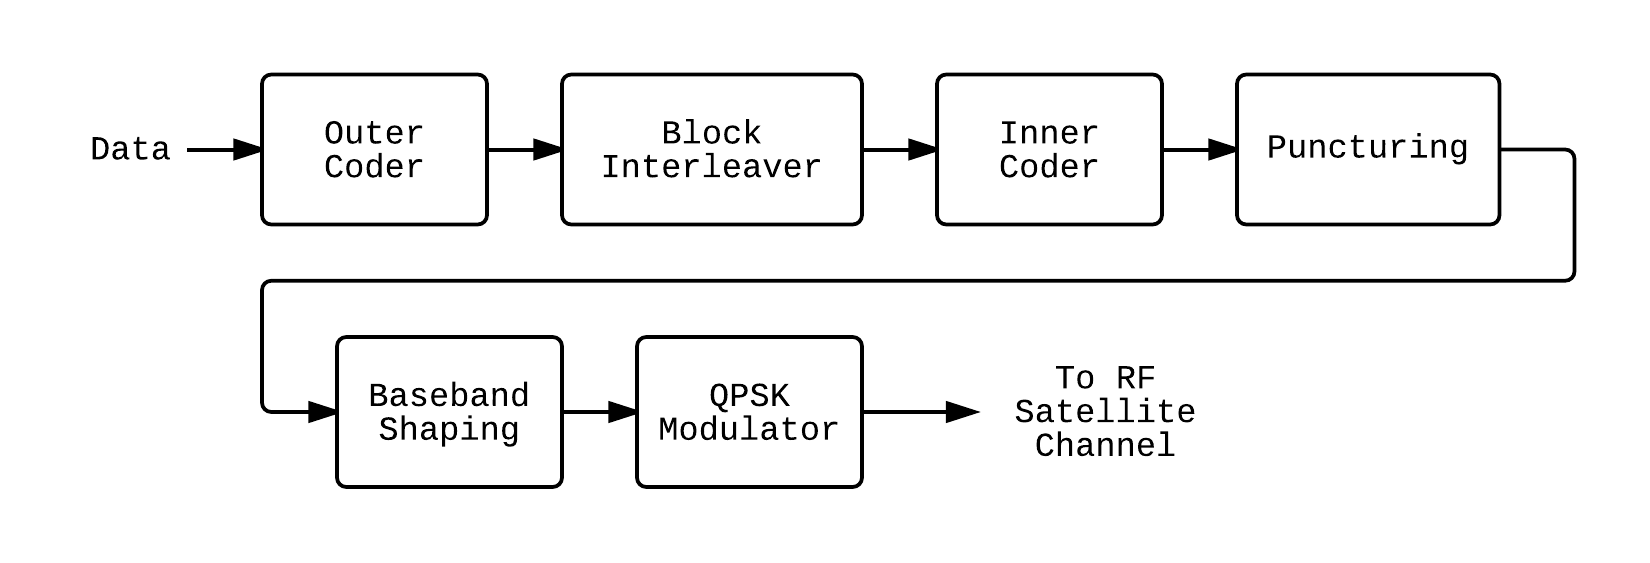
\includegraphics[scale=0.25]{EmitterL.png}
\caption{Emitter Architecture}\label{fig:TxArch}
\end{figure}

\begin{figure}[htb]
\centering
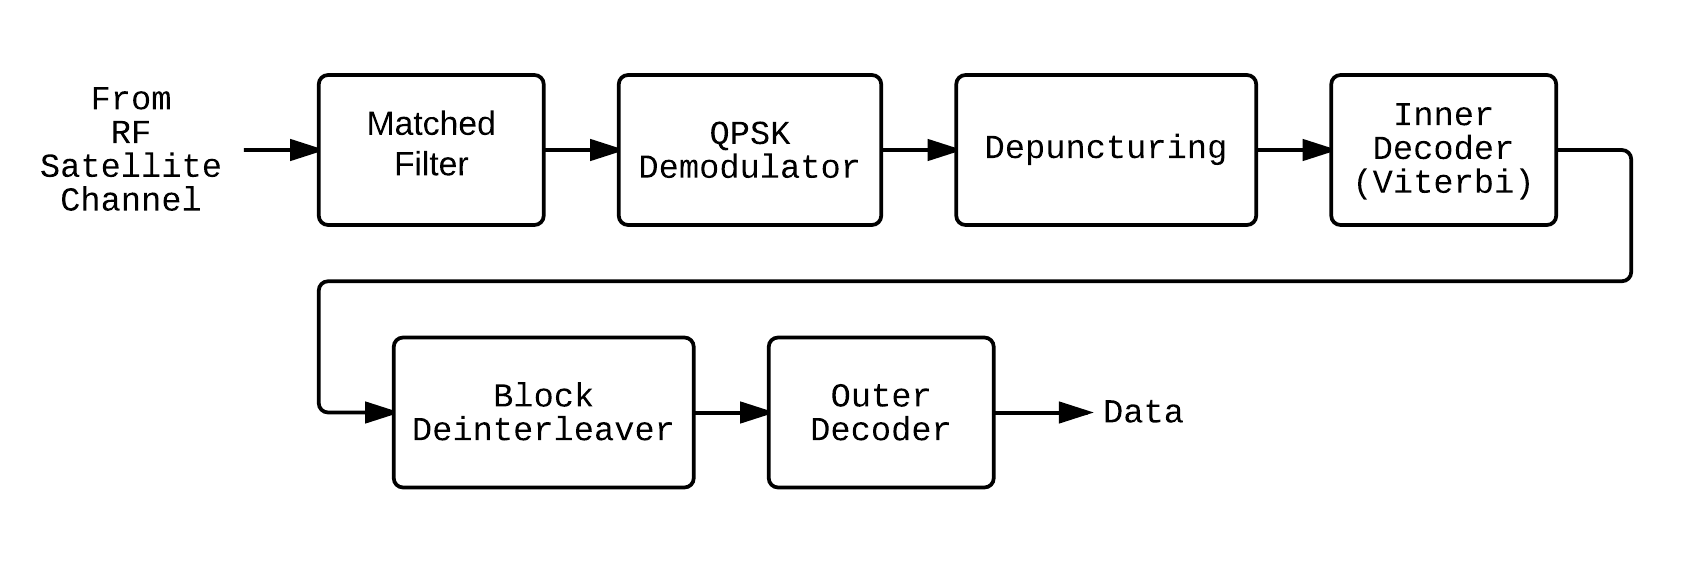
\includegraphics[scale=0.25]{ReceiverL.png}
\caption{Receiver Architecture}\label{fig:RxArch}
\end{figure}


\subsection{Outer Coding}

Outer coding is based on the shortened RS(204,188,T=8) code which in turn derives from an original RS(255,239,T=8). This shortening is achieved by adding 51 bytes, all set to zero, before the information bytes at the input of the (255,239) encoder. After the RS coding procedure these null bytes are discarded.

In order to protect transmissions from burst errors, a interleaver is added at the output of the outer encoder. Note that in this simulation a block interleaver is used while in the original DVB-S standard a convolutional interleaver. This allows the error bursts at the output of the inner decoder to be randomized in order to improve the burst error correction capabilities of the outer decoder.

\subsection{Inner Coding}

A range of punctured convolutional codes, based on a rate 1/2 convolutional code with constraint length K = 7 are possible. The selection of the most appropriate level of error correction for a given service is permitted this way. Possible codes allow with code rates of 1/2, 2/3, 3/4, 5/6 and 7/8. Generator polynomials are $g_1=171_{\text{oct}}$ and $g_2=133{\text{oct}}$ as defined in the standard. This corresponds to 64 possible trellis states. Simulations done will only include 2/3 puncturing using the puncturing matrix $P=[1 1 0 1]$. Decoding is done using a Viterbi decoder.

\subsection{Bit Mapping, Baseband Shaping and Modulation}

System uses conventional Gray-coded QPSK with absolute mapping. Prior to modulation, I and Q samples  (mathematically represented by a series of Dirac deltas, multiplied by the amplitudes I and Q, spaced by the symbol duration $T_s=1/R_s$ are square root raised cosine filtered. The roll-off factor is $\alpha=0.35$ and its frequency response is shown in Figure ~\ref{fig:txFilt}.

\begin{figure}[htb]
\centering
\includegraphics[scale=0.40]{matp_txfiltresp.eps}
\caption{Square root raised cosine filter with 35\% roll-off factor.}\label{fig:txFilt}
\end{figure}


\section{Simulation Results}

\subsection{Observed Signals}

First of all, let us take a look at the PSD of the transmitted signal (baseband). For this, Welch's method is used to estimate the power spectral density. The resulting PSD can be seen in Figure ~\ref{fig:TxPsd}.
\\

\begin{figure}[htb]
\centering
\includegraphics[scale=0.40]{matp_TxPsd.eps}
\caption{Transmitted signal's power spectrum density (PSD). Estimated using Welch's method.}\label{fig:TxPsd}
\end{figure}


\begin{figure}
\centering
\begin{subfigure}{.5\textwidth}
  \centering
  \includegraphics[width=1\linewidth]{matp_EyeClean.eps}
  \caption{No noise}
  \label{fig:eyeClean}
\end{subfigure}%
\begin{subfigure}{.5\textwidth}
  \centering
  \includegraphics[width=1\linewidth]{matp_Eye10dB.eps}
  \caption{$E_b/N_0 = 10\text{dB}$}
  \label{fig:eyeDirty}
\end{subfigure}
\caption{Eye diagrams at the output of the matched filter.}
\label{fig:eye}
\end{figure}

It is also interesting to generate some eye diagrams at the receiver side after matched filtering. This aids in determining the ideal sampling time as well as observing inter symbol interference (ISI). Figure ~\ref{fig:eye} shows two eye diagrams. Looking at the one were no noise is present we can see that there is effectively no ISI due to our Nyquist criterion fulfilling pulse shaping. Figure ~\ref{fig:Constellation} shows received and transmitted IQ samples.


\begin{figure}[htb]
\centering
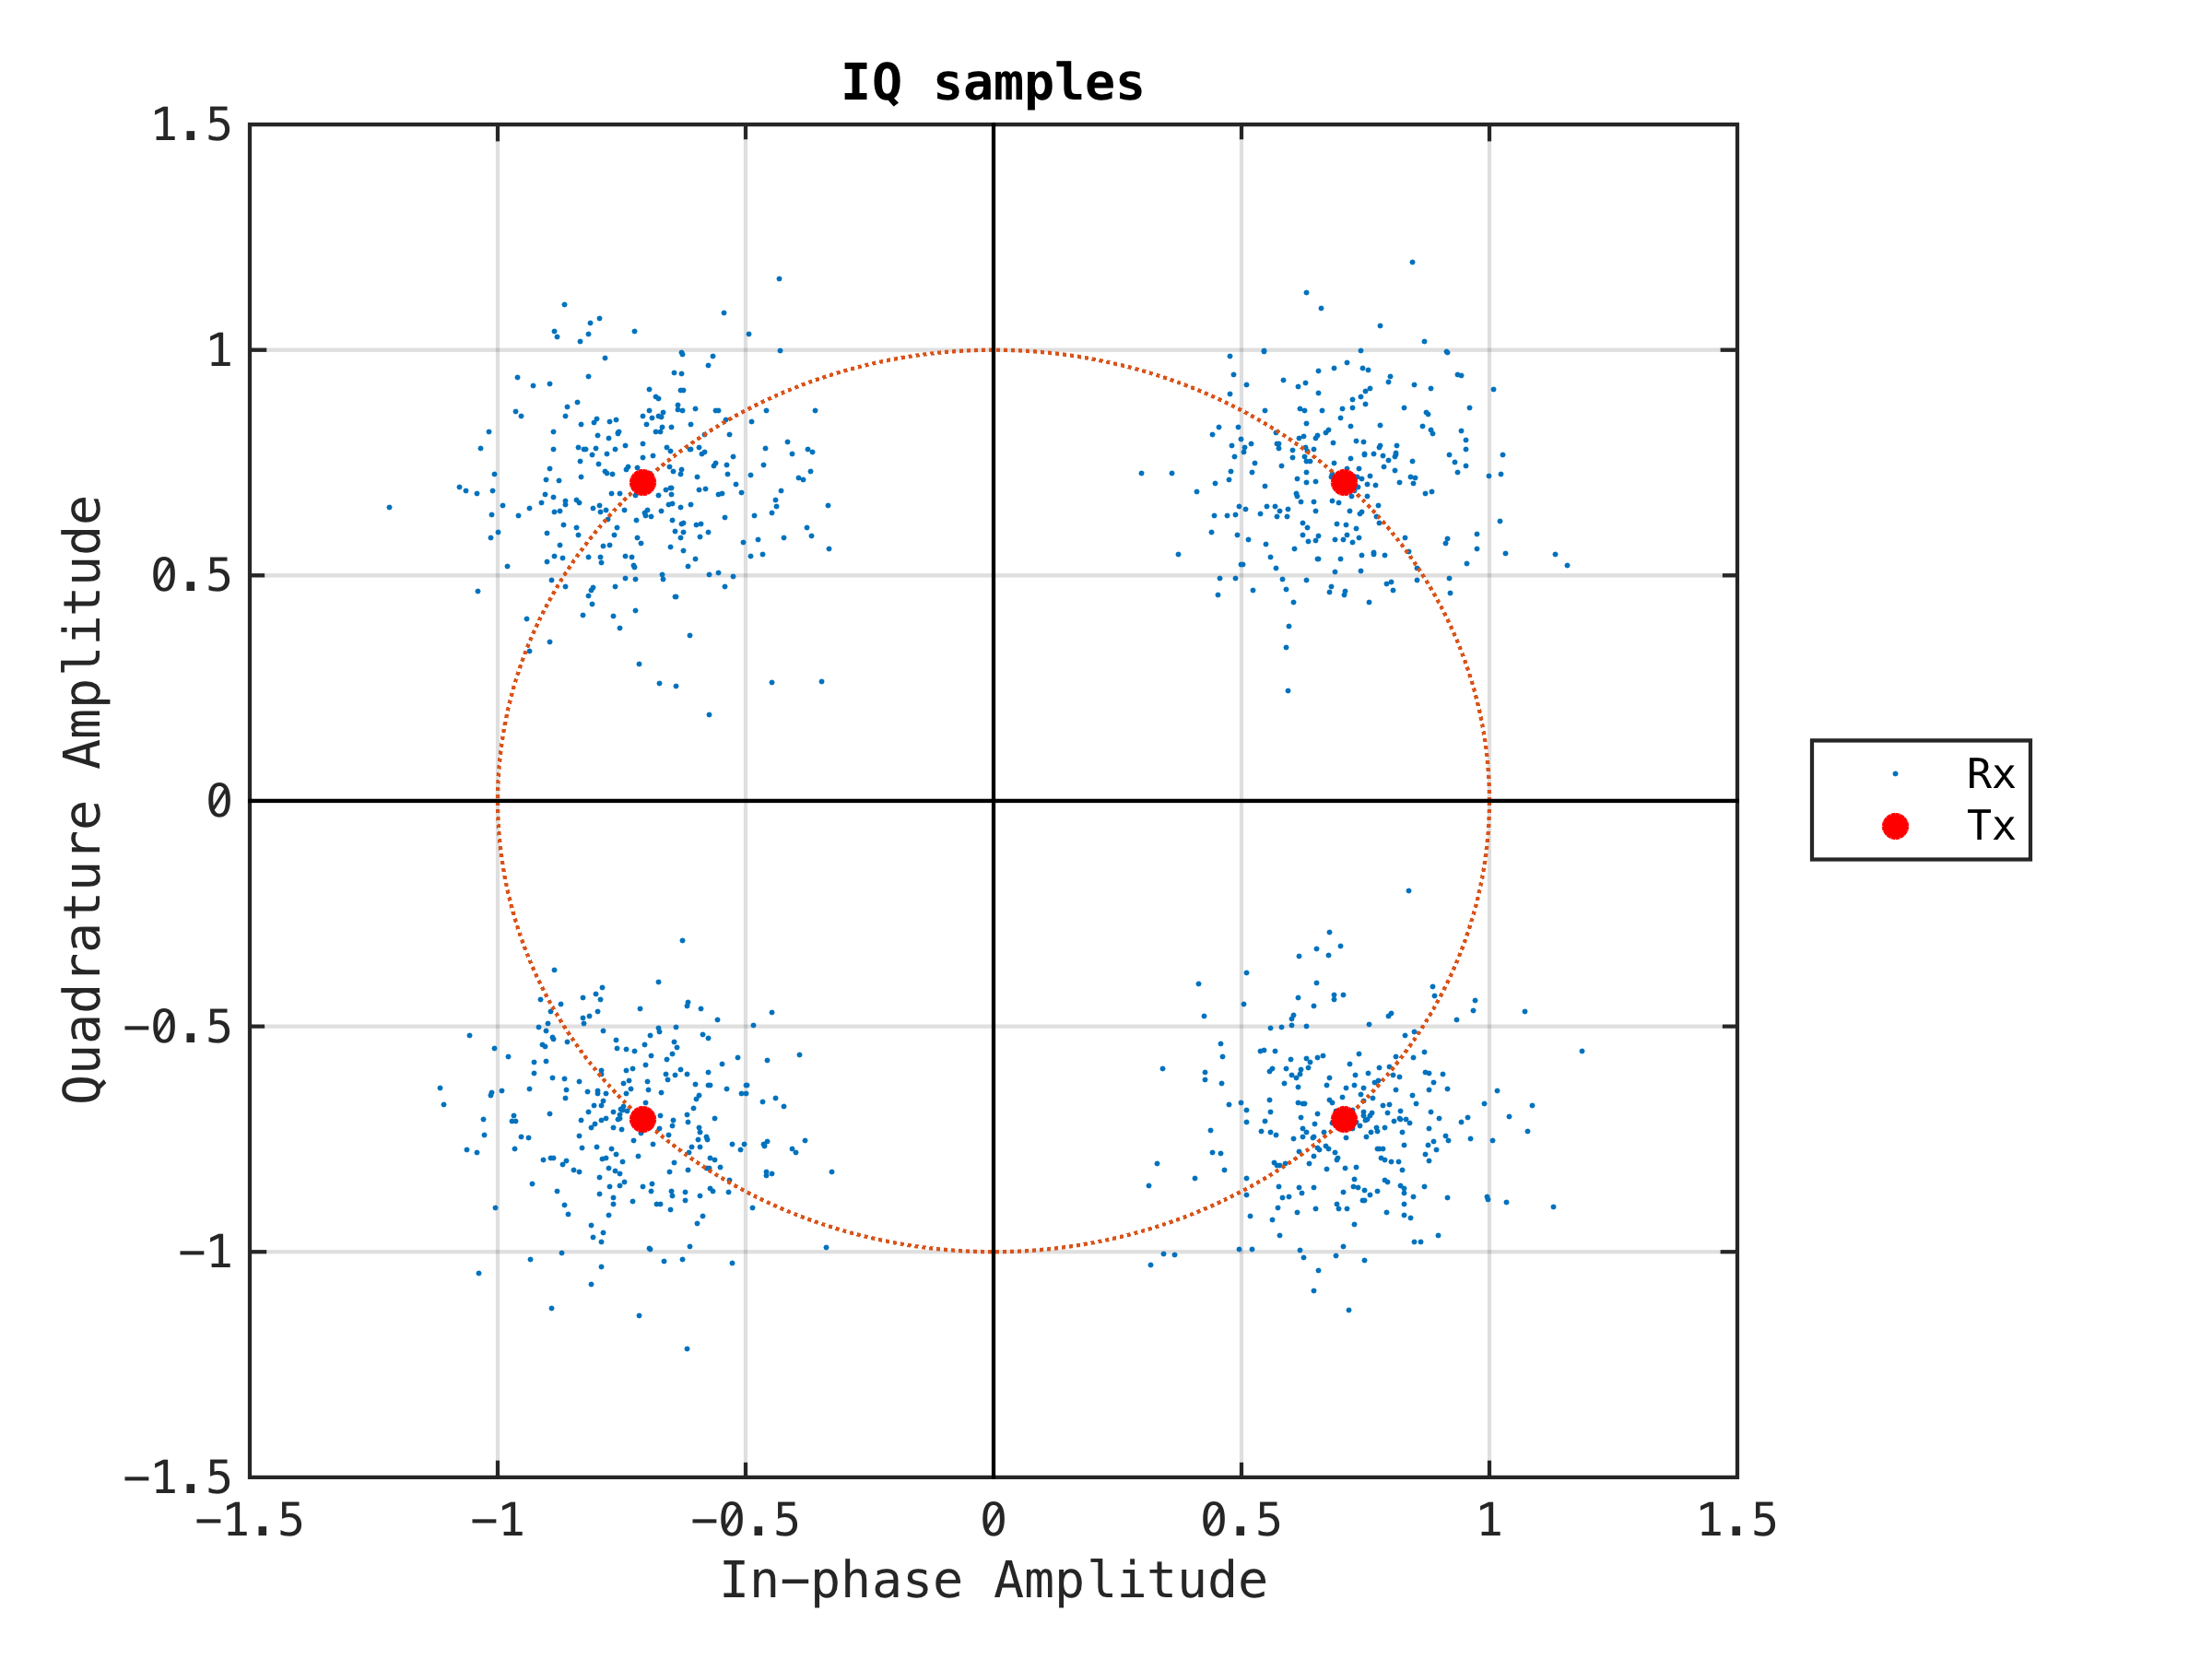
\includegraphics[scale=0.40]{matp_Constellation10dB.png}
\caption{Transmitted and received QPSK symbols with $E_b/N_0 = 10\text{dB}$  }\label{fig:Constellation}
\end{figure}


\subsection{BER Performance}

In order to validate the implementation, bit-error-rate (BER) performance is evaluated and compared against theoretical results. The expression for BER over an AWGN channel in QPSK without any coding is given by the following equation:

\begin{equation} \label{eq:qpskBer}
BER = Q\left(\sqrt{\frac{2E_b}{N_0}}\right)
\end{equation}

Where $E_b/N_0$ is the the energy per bit to noise power spectral density ratio. Various BER curves were derived utilizing different FEC configurations. Ultimately we computed the BER curve for the actual system with all FEC blocks enabled. These results can be seen in Figure ~\ref{fig:BER}. The labeling notation is as follows:


\begin{description}

  \item[No FEC, Theoretical] \hfill \\
  Theoretical QPSK over AWGN.
  \item[No FEC, Sim] \hfill \\
  Simulation with no forward error correction (FEC).
  \item[Convolutional Hard Decoder 1/2, Sim] \hfill \\
   Simulation with added 1/2 convolutional code and hard Viterbi decoder.
  \item[Convolutional Soft Decoder 1/2, Sim] \hfill \\
  Simulation with added 1/2 convolutional code and soft Viterbi decoder.
  \item[Convolutional Punctured 2/3, Sim] \hfill \\
  Simulation with punctured 2/3 convolutional code.
  \item[Reed Solomon 2/3, Sim] \hfill \\
  Simulation with punctured 2/3 convolutional inner coding as well as added Reed Solomon outer coding without block interleaving.
  \item[Reed Solomon Interleaved 2/3, Sim] \hfill \\
  Simulation with punctured 2/3 convolutional inner coding as well as added Reed Solomon outer coding with block interleaving of the outer encoder output (this is the system's actual BER curve).

\end{description}

\begin{figure}[htb]
\centering
\includegraphics[scale=0.40]{matp_BER.eps}
\caption{BER performance of different FEC configurations for Gray coded QPSK transmission over an AWGN channel. }\label{fig:BER}
\end{figure}

\subsubsection{QPSK over AWGN}

Observing both the theoretical as well as the simulated BER values when no type of coding is used, we can certainly validate the simulator implementation excluding of course all FEC related blocks.

\subsection{Convolutional Coding and Puncturing}


\subsection{Reed Solomon Coding and Interleaving}


%%% End document
\end{document}